

\chapter{Chapter Three}

\section{Event Comparisons}
Now, we consider each of the selected events individually, demonstrating that the events were
classified correctly, and breaking down the results from each case. Although it is nearly impossible to
extricate lake influence from synoptically classified events, synoptic-scale ascent is considered the
characterizing factor. Descriptions of the synoptic pattern during each event are given without
reference; For reference, see Appendix A for the 500mb Geopotential Heights, Skew-T charts, and
Sounding Climatology utilized. These descriptions are ancillary to the study and are provided to
demonstrate a variety of patterns are reresented.

\subsection{18 January 2014 - Synoptic}
In this event, a weak shortwave is approaching Southern Ontario as it rounds the base of a longwave
trough centered over the Eastern US. With the study area in the attendant
region of upper-level divergence, and a moist column present through 500mb, 
scattered snow showers form ahead of the shortwave. Figure \ref{fig:grid_ref_20140118} depicts
similiar cellular patterns between radars in the time-averaged $Z_{eH}$ field. In contrast, the $Z_{DR}$
comparison in Figure \ref{fig:grid_zdr_20140118}
shows that although the fields are similiar in their heterogenity, the spatial matching between the two is
tenuous everywhere but in the heaviest showers.

\begin{figure}[H]
\includegraphics[width=\textwidth]{grid/ref/20140118}
\caption{Gridded $Z_{eH}$ comparison for 18 January 2014. Time-average of all admitted scans.} 
\label{fig:grid_ref_20140118}
\end{figure}

\begin{figure}[H]
\includegraphics[width=\textwidth]{grid/zdr/20140118}
\caption{Gridded $Z_{DR}$ comparison for 18 January 2014. Time-average of all admitted scans.} 
\label{fig:grid_zdr_20140118}
\end{figure}
\vspace{5mm}

To investigate further, we examine a scatter-plot directly comparing matched values between radars.
Artifacts are present in both moments in Figure
\ref{fig:scatter_20140118}, indicated by evenly spaced vertical lines; these indicate an anomaly
originating from the axis of which they are normal to. For
$Z_{eH}$, Figure \ref{fig:scatter_ref_20140118} shows that artifacts are no longer present for values
greater than 15 dBZ, which indicates that a
stronger weather signal leads to better matching. On the contrary, Figure \ref{fig:scatter_zdr_20140118}
shows that for $Z_{DR}$, artifacts are present throughout. Also, the distribution of $Z_{DR}$ is unimodal. 

\begin{figure}[H]
\centering
   \begin{subfigure}{0.49\linewidth} \centering
     \includegraphics[scale=0.38]{scatter/ref/20140118}
     \caption{$Z_{eH}$ (dBZ)}\label{fig:scatter_ref_20140118}
   \end{subfigure}
   \begin{subfigure}{0.49\linewidth} \centering
     \includegraphics[scale=0.38]{scatter/zdr/20140118}
     \caption{$Z_{DR}$ (dB)}\label{fig:scatter_zdr_20140118}
   \end{subfigure}
\caption{Direct comparisons for 18 January 2014. Dataset includes all admitted grid cells.} \label{fig:scatter_20140118}
\end{figure}

It is still possible to extract a signal from the noise though, by only including data points with a
normalized kernel density estimate greater than or equal to two. These points are used to resolve the bias present in
$Z_{DR}$, as suggested by the comparisons. Figure \ref{fig:hist_20140118} gives an estimate of the
bias at CWKR by using this method and the known bias at KBUF as provided by the NEXRAD
External Target Bias Estimation technique. This method yields a median of -0.095 dB for the bias at CWKR, which when
considered with the error threshold of $\pm$0.1 dB, indicates no discernible bias.

\begin{figure}[H]
\includegraphics[width=0.75\textwidth]{hist/20140118}\centering
\caption{Histograms of $Z_{DR}$ (left), $Z_{DR}$ bias at CWKR, determined by subtracting the gridded, bias adjusted $Z_{DR}$ at KBUF from the $Z_{DR}$ at
CWKR. Both datasets include only matched points with KDE $\geq 2$. } 
\label{fig:hist_20140118}
\end{figure}



\begin{figure}[p]
\includegraphics[width=\textwidth]{grid/ref/20140123}
\caption{Gridded $Z_{eH}$ comparison for 23 January 2014. Time-average of all admitted scans.} 
\label{fig:grid_ref_20140123}
\end{figure}

\begin{figure}[p]
\includegraphics[width=\textwidth]{grid/zdr/20140123}
\caption{Gridded $Z_{DR}$ comparison for 23 January 2014. Time-average of all admitted scans.} 
\label{fig:grid_zdr_20140123}
\end{figure}

\subsection{23 January 2014 - Lake-Effect}
A positively tilted longwave trough dominates the eastern third of Canada during this event, with NW
winds at 850mb and SW winds at the surface. This light flow pattern yields the single, heavy
band depicted in Figure \ref{fig:grid_ref_20140123}, colloquially referred to as ``tea-kettle'' lake-effect
snow. There is also a background stream of very light lake-effect snow impinging from Lake Erie.
Spatial banding patterns of the lake-effect snow in the time-averaged $Z_{eH}$ fields as compared 
between the radars are remarkably similar. The difference between the grid mean values are within only
0.13 dBZ. In contrast, the $Z_{DR}$ comparison indicates that
although the fields are similiar in their heterogeniety, the spatial matching between the two is tenuous
everywhere but in the heaviest showers. An speckled pattern is also imparted on the $Z_{DR}$ fields
by the light snow from Lake Erie, evident in Figure \ref{fig:grid_zdr_20140123}. The scatter-plot in Figure \ref{fig:scatter_ref_20140123} shows an analysis
free of artifacts, and good agreement on average between radars. Although the agreement in $Z_{eH}$ between radars as
indicated by the orthonormal regression is acceptable, the chi-square
statistic indicates a high error variance. A slightly bi-modal distribution of $Z_{DR}$ is shown in 
Figure \ref{fig:scatter_ref_20140123}, with the main peak near 0 dB and a secondary peak near 0.5 dB, with artifacts much more prevalent near the secondary
peak. Both analysis methods have indicated a bias in $Z_{DR}$, so the
kernel density method for estimating bias is used. Figure \ref{fig:hist_20140123} shows an estimate of
the bias at CWKR, with a median value of -0.055 dB. Once again, no discernible bias exists outside of the error
threshold of $\pm$0.1 dB for this event.

\begin{figure}[H]
\centering
   \begin{subfigure}{0.49\linewidth} \centering
     \includegraphics[scale=0.38]{scatter/ref/20140123}
     \caption{$Z_{eH}$ (dBZ)}\label{fig:scatter_ref_20140123}
   \end{subfigure}
   \begin{subfigure}{0.49\linewidth} \centering
     \includegraphics[scale=0.38]{scatter/zdr/20140123}
     \caption{$Z_{DR}$ (dB)}\label{fig:scatter_zdr_20140123}
   \end{subfigure}
\caption{Direct comparisons for 23 January 2014. Dataset includes all admitted grid cells.}
\label{fig:scatter_20140123}
\end{figure}

\begin{figure}[H]
\includegraphics[width=0.75\textwidth]{hist/20140123}\centering
\caption{Histograms of $Z_{DR}$ (left), $Z_{DR}$ bias at CWKR, determined by subtracting the
gridded, bias adjusted $Z_{DR}$ at KBUF from the $Z_{DR}$ at CWKR. Both datasets include only
matched points with KDE $\geq 2$. } 
\label{fig:hist_20140123}
\end{figure}

\subsection{1 February 2014 - Synoptic}
This event is characterized by strong SW flow aloft, with above average moisture content. This leads to
widespread stratiform snow, with an eventual transition to rain outside of the time interval selected.
A large swath of steady snow is depicted by the time-averaged $Z_{eH}$ in Figure \ref{fig:grid_ref_20140201}. 
Furthermore, Figure \ref{fig:grid_zdr_20140201} shows smoother $Z_{DR}$
fields as compared with other events, which confirms the stratiform nature of the precipitation. Next, Figure \ref{fig:scatter_ref_20140201} indicates very
good agreement in $Z_{eH}$ with low error variance, while Figure \ref{fig:scatter_zdr_20140201} shows a very dense uni-modal, biased kernel for $Z_{DR}$. The
histogram in Figure \ref{fig:hist_20140201} reveals that the anomalous bias between the radars is indicative of a $Z_{DR}$ bias at CWKR, with a value of
0.217 dB. The source of this bias will be discussed in the next chapter.

\begin{figure}[H]
\includegraphics[width=\textwidth]{grid/ref/20140201}
\caption{Gridded $Z_{eH}$ comparison for 1 February 2014. Time-average of all admitted scans.} 
\label{fig:grid_ref_20140201}
\end{figure}

\begin{figure}[H]
\includegraphics[width=\textwidth]{grid/zdr/20140201}
\caption{Gridded $Z_{DR}$ comparison for 1 February 2014. Time-average of all admitted scans.} 
\label{fig:grid_zdr_20140201}
\end{figure}

\begin{figure}[H]
\centering
   \begin{subfigure}{0.49\linewidth} \centering
     \includegraphics[scale=0.38]{scatter/ref/20140201}
     \caption{$Z_{eH}$ (dBZ)}\label{fig:scatter_ref_20140201}
   \end{subfigure}
   \begin{subfigure}{0.49\linewidth} \centering
     \includegraphics[scale=0.38]{scatter/zdr/20140201}
     \caption{$Z_{DR}$ (dB)}\label{fig:scatter_zdr_20140201}
   \end{subfigure}
\caption{Direct comparisons for 1 February 2014. Dataset includes all admitted grid cells.} \label{fig:scatter_20140201}
\end{figure}

\begin{figure}[H]
\includegraphics[width=0.75\textwidth]{hist/20140201}\centering
\caption{Histograms of $Z_{DR}$ (left), $Z_{DR}$ bias at CWKR, determined by subtracting the gridded, bias adjusted $Z_{DR}$ at KBUF from the $Z_{DR}$ at
CWKR. Both datasets include only matched points with KDE $\geq 2$. } 
\label{fig:hist_20140201}
\end{figure}

\subsection{6 January 2015 - Lake-Effect}
A highly zonal, NW flow aloft is present in this case, a typical pattern for lake-effect snow across the Great Lakes region. Anemic in radar appearance, a
lake-effect band develops in the light winds near the surface; this case could be characterized as a weak ``tea-kettle'' event. Figure
\ref{fig:grid_ref_20150106} depicts stationary banding in the time-averaged $Z_{eH}$. Of note is that CWKR observes more of the finer scale features as
compared with KBUF, also evidenced by the +2.9 dBZ difference in $Z_{eH}$ mean. 
\begin{figure}[H]
\includegraphics[width=\textwidth]{grid/ref/20150106}
\caption{Gridded $Z_{eH}$ comparison for 6 January 2015. Time-average of all admitted scans.} 
\label{fig:grid_ref_20150106}
\end{figure}
This case stands out from the rest in terms of $Z_{DR}$, as the fields are
very similiar and unbiased as shown in Figure \ref{fig:grid_zdr_20150106}. The scatter-plot in Figure
\ref{fig:scatter_ref_20150106} confirms what is shown in the gridded $Z_{eH}$, with values skewed higher for CWKR. Figure \ref{fig:scatter_zdr_20150106}
shows a bi-modal distribution for $Z_{DR}$, with the
main peak around 0.5 dB and a secondary peak near 0 dB. The histogram in Figure
\ref{fig:hist_20150106} confirms the observed unbiased $Z_{DR}$, with a near zero median value of 0.003 dB.


\begin{figure}[H]
\includegraphics[width=\textwidth]{grid/zdr/20150106}
\caption{Gridded $Z_{DR}$ comparison for 6 January 2015. Time-average of all admitted scans.} 
\label{fig:grid_zdr_20150106}
\end{figure}

\begin{figure}[H]
\centering
   \begin{subfigure}{0.49\linewidth} \centering
     \includegraphics[scale=0.38]{scatter/ref/20150106}
     \caption{$Z_{eH}$ (dBZ)}\label{fig:scatter_ref_20150106}
   \end{subfigure}
   \begin{subfigure}{0.49\linewidth} \centering
     \includegraphics[scale=0.38]{scatter/zdr/20150106}
     \caption{$Z_{DR}$ (dB)}\label{fig:scatter_zdr_20150106}
   \end{subfigure}
\caption{Direct comparisons for 6 January 2015. Dataset includes all admitted grid cells.} \label{fig:scatter_20150106}
\end{figure}

\begin{figure}[H]
\includegraphics[width=0.75\textwidth]{hist/20150106}\centering
\caption{Histograms of $Z_{DR}$ (left), $Z_{DR}$ bias at CWKR, determined by subtracting the gridded, bias adjusted $Z_{DR}$ at KBUF from the $Z_{DR}$ at
CWKR. Both datasets include only matched points with KDE $\geq 2$. } 
\label{fig:hist_20150106}
\end{figure}

\subsection{7 January 2015 - Synoptic}
Less than 24 hours after the previous event, the zonal flow has buckled and a strong shortwave is overhead Southern Ontario. Radar animations indicate a
frontally forced band of snow showers. Figure \ref{fig:grid_ref_20150107} shows the solid band of snow progressed from mid-lake southward, with similiar
depictions of $Z_{eH}$ between radars. Inspection of the scatter-plot in Figure \ref{fig:scatter_ref_20150107} indicates good agreement with reasonable error
variance, while Figure \ref{fig:scatter_zdr_20150107} shows a uni-modal distribution of $Z_{DR}$ with a relatively dense kernel.
Meanwhile, Figure \ref{fig:grid_zdr_20150107} shows two heterogenous fields, especially noisy in areas of light returns. 
Estimating the bias at CWKR, the histogram in Figure \ref{fig:hist_20150107} gives a median value of -0.040 dB. This indicates that no discernible bias
exists outside of the error threshold of $\pm$0.1 dB for this event.

\begin{figure}[H]
\includegraphics[width=\textwidth]{grid/ref/20150107}
\caption{Gridded $Z_{eH}$ comparison for 7 January 2015. Time-average of all admitted scans.} 
\label{fig:grid_ref_20150107}
\end{figure}

\begin{figure}[H]
\includegraphics[width=\textwidth]{grid/zdr/20150107}
\caption{Gridded $Z_{DR}$ comparison for 7 January 2015. Time-average of all admitted scans.} 
\label{fig:grid_zdr_20150107}
\end{figure}
\begin{figure}[H]
\centering
   \begin{subfigure}{0.49\linewidth} \centering
     \includegraphics[scale=0.38]{scatter/ref/20150107}
     \caption{$Z_{eH}$ (dBZ)}\label{fig:scatter_ref_20150107}
   \end{subfigure}
   \begin{subfigure}{0.49\linewidth} \centering
     \includegraphics[scale=0.38]{scatter/zdr/20150107}
     \caption{$Z_{DR}$ (dB)}\label{fig:scatter_zdr_20150107}
   \end{subfigure}
\caption{Direct comparisons for 7 January 2015. Dataset includes all admitted grid cells.} \label{fig:scatter_20150107}
\end{figure}

\begin{figure}[H]
\includegraphics[width=0.75\textwidth]{hist/20150107}\centering
\caption{Histograms of $Z_{DR}$ (left), $Z_{DR}$ bias at CWKR, determined by subtracting the gridded, bias adjusted $Z_{DR}$ at KBUF from the $Z_{DR}$ at
CWKR. Both datasets include only matched points with KDE $\geq 2$. } 
\label{fig:hist_20150107}
\end{figure}

\subsection{6 February 2015 - Synoptic}
With a strong ridge centered over the SW US, Southern Ontario is on the backside of progressive shortwave, with a frontal passage occuring once again. A
broad swath of snow is depicted by the time-averaged $Z_{eH}$ fields in Figure \ref{fig:grid_ref_20150206}, with the CWKR mean value 2 dBZ higher than KBUF.
\begin{figure}[H]
\includegraphics[width=\textwidth]{grid/ref/20150206}
\caption{Gridded $Z_{eH}$ comparison for 6 February 2015. Time-average of all admitted scans.} 
\label{fig:grid_ref_20150206}
\end{figure}
Comparing $Z_{DR}$ as shown in Figure \ref{fig:grid_zdr_20150206}, the fields are similiar but slightly biased. Beam blockages are noted at CWKR as indicated
by the stripes in the NE section of grid. Next to the scatter-plots, with Figure \ref{fig:scatter_20150206} indicating a high
frequency of points between 15-25 dBZ, a preferred range for comparing $Z_{DR}$ values. Also of note is the high error variance of 9.773 .
Figure \ref{fig:scatter_zdr_20150206} shows a dense, symmetric kernel with an ill-fitted regression. Proceeding on to the histograms in Figure
\ref{fig:hist_20150206}, a median bias of 0.283 dB at CWKR is estimated. The source of the bias will be discussed in the next chapter. 

\begin{figure}[p]
\includegraphics[width=\textwidth]{grid/zdr/20150206}
\caption{Gridded $Z_{DR}$ comparison for 6 February 2015. Time-average of all admitted scans.} 
\label{fig:grid_zdr_20150206}
\end{figure}

\begin{figure}[p]
\centering
   \begin{subfigure}{0.49\linewidth} \centering
     \includegraphics[scale=0.38]{scatter/ref/20150206}
     \caption{$Z_{eH}$ (dBZ)}\label{fig:scatter_ref_20150206}
   \end{subfigure}
   \begin{subfigure}{0.49\linewidth} \centering
     \includegraphics[scale=0.38]{scatter/zdr/20150206}
     \caption{$Z_{DR}$ (dB)}\label{fig:scatter_zdr_20150206}
   \end{subfigure}
\caption{Direct comparisons for 6 February 2015. Dataset includes all admitted grid cells.} \label{fig:scatter_20150206}
\end{figure}

\begin{figure}[H]
\includegraphics[width=0.75\textwidth]{hist/20150206}\centering
\caption{Histograms of $Z_{DR}$ (left), $Z_{DR}$ bias at CWKR, determined by subtracting the gridded, bias adjusted $Z_{DR}$ at KBUF from the $Z_{DR}$ at
CWKR. Both datasets include only matched points with KDE $\geq 2$. } 
\label{fig:hist_20150206}
\end{figure}

\subsection{14 February 2015 - Lake-Effect}
While Southern Ontario is bracing for the impact of a bowling-ball like lobe of the polar vortex, strong W to SW flow from the surface to 850mb allows for a prolonged period of lake-effect snow over the lake. From Figure \ref{fig:grid_ref_20150214}, we see again that CWKR resolves the convective scale features of the snow squalls better than KBUF. Horizontal convective rolls are clearly depicted by CWKR, whereas they become muddled by KBUF. Figure \ref{fig:grid_zdr_20150214} shows similiar patterns of $Z_{DR}$, but a large bias exists. The $Z_{eH}$ scatter-plot in Figure \ref{fig:scatter_20150214} shows a dense clustering of points for low values, becoming increasingly skewed towards CWKR as they increase. For $Z_{DR}$, the variance-weighted regression achieves a near perfect reduced chi statistic ($\chi^2_\nu$) of 0.968. The histogram in Figure \ref{fig:hist_20150214} indicates a anomalous bias for this event, with a median value of 0.377 dB.

\begin{figure}[p]
\includegraphics[width=\textwidth]{grid/ref/20150214}
\caption{Gridded $Z_{eH}$ comparison for 14 February 2015. Time-average of all admitted scans.} 
\label{fig:grid_ref_20150214}
\end{figure}

\begin{figure}[p]
\includegraphics[width=\textwidth]{grid/zdr/20150214}
\caption{Gridded $Z_{DR}$ comparison for 14 February 2015. Time-average of all admitted scans.} 
\label{fig:grid_zdr_20150214}
\end{figure}

\begin{figure}[p]
\centering
   \begin{subfigure}{0.49\linewidth} \centering
     \includegraphics[scale=0.38]{scatter/ref/20150214}
     \caption{$Z_{eH}$ (dBZ)}\label{fig:scatter_ref_20150214}
   \end{subfigure}
   \begin{subfigure}{0.49\linewidth} \centering
     \includegraphics[scale=0.38]{scatter/zdr/20150214}
     \caption{$Z_{DR}$ (dB)}\label{fig:scatter_zdr_20150214}
   \end{subfigure}
\caption{Direct comparisons for 14 February 2015. Dataset includes all admitted grid cells.} \label{fig:scatter_20150214}
\end{figure}

\begin{figure}[p]
\includegraphics[width=0.75\textwidth]{hist/20150214}\centering
\caption{Histograms of $Z_{DR}$ (left), $Z_{DR}$ bias at CWKR, determined by subtracting the gridded, bias adjusted $Z_{DR}$ at KBUF from the $Z_{DR}$ at CWKR. Both datasets include only matched points with KDE $\geq 2$. } 
\label{fig:hist_20150214}
\end{figure}

\subsection{18 February 2015 - Lake-Effect}
Four days later, The polar vortex has arrived in earnest for this event, with the 500 dm isoheight at 500mb nearing as far south as Windsor, ON. The cold airmass allows for the development of an intense lake-effect snow band, the strongest of all the lake-effect cases as indicated by the $Z_{eH}$ means in Figure \ref{fig:grid_ref_20150218}. Next, Figure \ref{fig:grid_zdr_20150218} shows similiar band structure as compared between radars, with a bias evident. A orthonormal fit with decent agreement between radars is shown in Figure \ref{fig:scatter_ref_20150218}, with the values biased towards CWKR all along the line. In Figure \ref{fig:scatter_zdr_20150218}, a unique bi-modal distribution of $Z_{DR}$ is shown, with two peaks equal in magnitude around 0.50 dB and 0.75 dB. The histogram in Figure \ref{fig:hist_20150218} also depicts this bi-modal distribution of $Z_{DR}$, and gives an estimate median value of 0.296 dB. The source of the bias will be discussed in the next chapter. 
\begin{figure}[H]
\includegraphics[width=\textwidth]{grid/ref/20150218}
\caption{Gridded $Z_{eH}$ comparison for 18 February 2015. Time-average of all admitted scans.} 
\label{fig:grid_ref_20150218}
\end{figure}

\begin{figure}[p]
\includegraphics[width=\textwidth]{grid/zdr/20150218}
\caption{Gridded $Z_{DR}$ comparison for 18 February 2015. Time-average of all admitted scans.} 
\label{fig:grid_zdr_20150218}
\end{figure}

\begin{figure}[p]
\centering
   \begin{subfigure}{0.49\linewidth} \centering
     \includegraphics[scale=0.38]{scatter/ref/20150218}
     \caption{$Z_{eH}$ (dBZ)}\label{fig:scatter_ref_20150218}
   \end{subfigure}
   \begin{subfigure}{0.49\linewidth} \centering
     \includegraphics[scale=0.38]{scatter/zdr/20150218}
     \caption{$Z_{DR}$ (dB)}\label{fig:scatter_zdr_20150218}
   \end{subfigure}
\caption{Direct comparisons for 18 February 2015. Dataset includes all admitted grid cells.} \label{fig:scatter_20150218}
\end{figure}

\begin{figure}[H]
\includegraphics[width=0.75\textwidth]{hist/20150218}\centering
\caption{Histograms of $Z_{DR}$ (left), $Z_{DR}$ bias at CWKR, determined by subtracting the gridded, bias adjusted $Z_{DR}$ at KBUF from the $Z_{DR}$ at
CWKR. Both datasets include only matched points with KDE $\geq 2$. } 
\label{fig:hist_20150218}
\end{figure}

\subsection{10 February 2016 - Lake-Effect}
The 500mb ridge axis is centered to the south of Southern Ontario in the Appalachians, with WNW flow aloft during this event. With a slight amount of pre
existing instability augmenting the lake induced instabilities, a healthly band of lake-effect snow forms on the southern end of the lake. KBUF observes
higher values of $Z_{DR}$ in this band on the southern edge of the lake, as shown in Figure \ref{fig:grid_ref_20160210}. This is likely due to the CWKR beam
overshooting the shallow convection while the KBUF beam is lower in height. The intensity of the band overcomes the degraded signal strength due beam
blockages at CWKR, evident in $Z_{DR}$ on the western end of the band in Figure \ref{fig:grid_zdr_20160210}. 
\begin{figure}[H]
\includegraphics[width=\textwidth]{grid/ref/20160210}
\caption{Gridded $Z_{eH}$ comparison for 10 February 2016. Time-average of all admitted scans.} 
\label{fig:grid_ref_20160210}
\end{figure}

\begin{figure}[H]
\includegraphics[width=\textwidth]{grid/zdr/20160210}
\caption{Gridded $Z_{DR}$ comparison for 10 February 2016. Time-average of all admitted scans.} 
\label{fig:grid_zdr_20160210}
\end{figure}

\vspace{5mm}

Due to the long duration of this case, the large
sample of matched points was obtained from this case. Figure \ref{fig:scatter_ref_20160210} shows that matched $Z_{eH}$ values tends higher towards KBUF as
they increase. Next, Figure \ref{fig:scatter_zdr_20160210} demonstrates the value of the kernel density estimate, as its impossible to visually analyze a
scatter-plot with nearly a million points. The kernel extracted from the data is small, but information rich. Figure \ref{fig:hist_20160210} leverages this
information to show that the median $Z_{DR}$ at CWKR is -0.055 dB, indicating no discernible bias exists outside of the error threshold of $\pm$0.1 dB for
this event.

\begin{figure}[H]
\centering
   \begin{subfigure}{0.49\linewidth} \centering
     \includegraphics[scale=0.38]{scatter/ref/20160210}
     \caption{$Z_{eH}$ (dBZ)}\label{fig:scatter_ref_20160210}
   \end{subfigure}
   \begin{subfigure}{0.49\linewidth} \centering
     \includegraphics[scale=0.38]{scatter/zdr/20160210}
     \caption{$Z_{DR}$ (dB)}\label{fig:scatter_zdr_20160210}
   \end{subfigure}
\caption{Direct comparisons for 10 February 2016. Dataset includes all admitted grid cells.} \label{fig:scatter_20160210}
\end{figure}

\begin{figure}[H]
\includegraphics[width=0.75\textwidth]{hist/20160210}\centering
\caption{Histograms of $Z_{DR}$ (left), $Z_{DR}$ bias at CWKR, determined by subtracting the gridded, bias adjusted $Z_{DR}$ at KBUF from the $Z_{DR}$ at
CWKR. Both datasets include only matched points with KDE $\geq 2$. } 
\label{fig:hist_20160210}
\end{figure}

\subsection{15 December 2016 - Synoptic}
A deep longwave trough is centered over Southern Ontario, with an Arctic airmass in place over the Great Lakes region. With meager moisture in place, a
post-frontal trough manages to squeeze out some passing snow-showers. As indicated by Figure \ref{fig:grid_ref_20161215}, the spatial patterns of $Z_{eH}$ are in very good agreement. In contrast, Figure \ref{fig:grid_zdr_20161215} shows two very noisy $Z_{DR}$ fields. Even with the small sample size, Figure \ref{fig:scatter_20161215} shows that decent fits are achieved for both moments. Meanwhile, the histogram in Figure \ref{fig:hist_20161215} shows that the estimate of bias at CWKR is large, with a median value of -0.465 dB. This case is an outlier; the source of this large bias will be discussed in the next chapter. 
\begin{figure}[p]
\includegraphics[width=\textwidth]{grid/ref/20161215}
\caption{Gridded $Z_{eH}$ comparison for 15 December 2016. Time-average of all admitted scans.} 
\label{fig:grid_ref_20161215}
\end{figure}

\begin{figure}[p]
\includegraphics[width=\textwidth]{grid/zdr/20161215}
\caption{Gridded $Z_{DR}$ comparison for 15 December 2016. Time-average of all admitted scans.} 
\label{fig:grid_zdr_20161215}
\end{figure}

\begin{figure}[p]
\centering
   \begin{subfigure}{0.49\linewidth} \centering
     \includegraphics[scale=0.38]{scatter/ref/20161215}
     \caption{$Z_{eH}$ (dBZ)}\label{fig:scatter_ref_20161215}
   \end{subfigure}
   \begin{subfigure}{0.49\linewidth} \centering
     \includegraphics[scale=0.38]{scatter/zdr/20161215}
     \caption{$Z_{DR}$ (dB)}\label{fig:scatter_zdr_20161215}
   \end{subfigure}
\caption{Direct comparisons for 15 December 2016. Dataset includes all admitted grid cells.} \label{fig:scatter_20161215}
\end{figure}

\begin{figure}[p]
\includegraphics[width=0.75\textwidth]{hist/20161215}\centering
\caption{Histograms of $Z_{DR}$ (left), $Z_{DR}$ bias at CWKR, determined by subtracting the gridded, bias adjusted $Z_{DR}$ at KBUF from the $Z_{DR}$ at
CWKR. Both datasets include only matched points with KDE $\geq 2$. } 
\label{fig:hist_20161215}
\end{figure}

\section{$Z_{eH}$ Subset Comparisons}
Now that all the cases have been presented individually, two subsets are created for comparison. The first consists of the five lake-effect events, the
subset of interest, as compared with the five synoptic events, which act as a control subset.
A comparison of these subset is shown in Figure \ref{fig:ref_scatter}, with a scatter-plot of KBUF $Z_{eH}$ data versus CWKR on the common grid. Figure
\ref{fig:ref_synoptic} is the subset of synoptic events while Figure \ref{fig:ref_lake_effect} is the subset of lake-effect events. These results show that
comparable performance between radars is achieved in lake-effect events. An interesting result is the clustering of points for the range $0 < Z_{eH} < 10$ dBZ in lake-effect events. This is in contrast with the higher clustering of points in synoptic events, from $10 < Z_{eH} < 25$. This could indicate that KBUF is underestimating $Z_{eH}$ in shallow lake-effect events, at the slope of regression is 0.94, as compared with 1.01 for synoptic events.

\begin{figure}[H]
\centering
   \begin{subfigure}{0.49\linewidth} \centering
     \includegraphics[scale=0.45]{ref_scatter_synoptic}
     \caption{subset of synoptic snow events}\label{fig:ref_synoptic}
   \end{subfigure}
   \begin{subfigure}{0.49\linewidth} \centering
     \includegraphics[scale=0.45]{ref_scatter_lake_effect}
     \caption{subset of lake-effect snow events}\label{fig:ref_lake_effect}
   \end{subfigure}
\caption{Scatter-plots of CWKR versus KBUF grid analyzed reflectivity, with Kernel Density Estimation shading. The red line is an Orthonormal Linear
Regression, with a black identity line.} \label{fig:ref_scatter}
\end{figure}

\section{KDE Constrained $Z_{DR}$}
The next step is to demonstrate the usefulness of constraining the datasets with a KDE threshold. The
constrained $Z_{DR}$ datasets represent the areas where both radars indicate a higher likelihood of
representing the true bulk hydrometeor type present in any given volume. An interpretation of the
hydrometeors present can then be made, based on the range of values found in the constrained set. All
cases are presented in chronological order.
\subsection{Unbiased $Z_{DR}$ Cases}
Cases where the calculated $Z_{DR}$ bias at CWKR did not exceed the error threshold of $\pm$ 0.1 dB are presented first, without any bias adjustment made.
\subsubsection{18 January 2014}
The first unbiased case in Figure \ref{fig:grid_zdr_kde_20140118} shows how the constrainment highlights the cells that passed through the eastern side of the domain. Areas of higher $Z_{eH}$  are correlated with the constrained $Z_{DR}$ areas, indicating that dataset is distilled down to include only returns with higher signal-to-noise-ratio (SNR) values. $Z_{DR}$ values closer to 0.50 dB in this case indicate that less aggregation is occurring and more pristine crystals are present.
\begin{figure}[H]
\includegraphics[width=\textwidth]{grid/zdr_kde/20140118}
\caption{Comparison of gridded $Z_{DR}$ with Gaussian smoothed contours of $Z_{eH}$ for 18 January 2014. $Z_{DR}$ is constrained by only including points with a
KDE $\geq 2$.}
\label{fig:grid_zdr_kde_20140118}
\end{figure}
\subsubsection{23 January 2014}
The next case in Figure \ref{fig:grid_zdr_kde_20140123} also shows the advantage of the constrainment, in that it delineates the banding pattern present in this case. Furthermore, the partial beam blockages present in the unconstrained dataset are removed. Both radars agree that this intense snow
squall is generating dry aggregated snow, with $Z_{DR}$ values in the characteristic range of 0-0.2 dB.
\begin{figure}[H]
\includegraphics[width=\textwidth]{grid/zdr_kde/20140123}
\caption{Comparison of gridded $Z_{DR}$ with Gaussian smoothed contours of $Z_{eH}$ for 23 January 2014. $Z_{DR}$ is constrained by only including points with a
$KDE \geq 2$.} 
\label{fig:grid_zdr_kde_20140123}
\end{figure}
\subsubsection{6 January 2015}
The 6 January 2015 case shown in Figure \ref{fig:grid_zdr_kde_20150106} shows remarkably similiar fields for both variables. This is likely due to the extremely shallow nature of the snow-squall, with a mean max echo top of 0.46 km. Another feature shown is the high amount of points excluded in high $Z_{eH}$ areas,  i.e. inside the 20 dBZ contour. Looking back at Figure \ref{fig:grid_zdr_20150106}, even with very similiar mean values of $Z_{DR}$, CWKR reports much higher values in this area. It is likely that large, spherical aggregates were occurring inside this 20 dBZ contour. As these large particles approach the C-Band wavelength of 5 cm, they could be inducing resonance effects; this type of resonance effect has been observed by \citet{Hassan2017}.
\begin{figure}[H]
\includegraphics[width=\textwidth]{grid/zdr_kde/20150106}
\caption{Comparison of gridded $Z_{DR}$ with Gaussian smoothed contours of $Z_{eH}$ for 6 January 2014. $Z_{DR}$ is constrained by only including points with a
KDE $\geq 2$.} 
\label{fig:grid_zdr_kde_20150106}
\end{figure}
\subsubsection{7 January 2015}
Once again, as shown in Figure \ref{fig:grid_zdr_kde_20150107}, excellent delineation of precipitating structures is achieved through this method. No obvious pattern emerges within the higher $Z_{DR}$, with values varying tightly around 0.2 dB. Of note are the higher $Z_{DR}$ values on the edge of the heavier precipitation shield as reported by KBUF, with CWKR not reporting these higher values. This could be due to unequal beam broadening between radars.
\begin{figure}[H]
\includegraphics[width=\textwidth]{grid/zdr_kde/20150107}
\caption{Comparison of gridded $Z_{DR}$ with Gaussian smoothed contours of $Z_{eH}$ for 7 January 2014. $Z_{DR}$ is constrained by only including points with a
KDE $\geq 2$.} 
\label{fig:grid_zdr_kde_20150107}
\end{figure}

\subsubsection{10 February 2016}
A much more subtle gradient from censored to admitted points is present in Figure \ref{fig:grid_zdr_kde_20160210}. $Z_{DR}$ values are right around 0 dB for this case, which indicates spherical aggregates are dominating. This event has the warmest surface temperature, with the 12Z Buffalo sounding reporting $-2.7^{\circ}$ C. Warmer temperatures closer to $0^{\circ}$ C are conducive for this type of aggregation process \citep{Hosler1957}. 
\begin{figure}[H]
\includegraphics[width=\textwidth]{grid/zdr_kde/20160210}
\caption{Comparison of gridded $Z_{DR}$ with Gaussian smoothed contours of $Z_{eH}$ for 10 February 2016. $Z_{DR}$ is constrained by only including points with a
KDE $\geq 2$.} 
\label{fig:grid_zdr_kde_20160210}
\end{figure}

\subsection{Biased $Z_{DR}$ Cases}
Cases where the calculated $Z_{DR}$ bias at CWKR exceeded the error threshold of $\pm$ 0.1 dB are presented next, with the previously calculated median bias used to adjust $Z_{DR}$ values at CWKR.
\subsubsection{1 February 2014}
The first biased case shown in Figure \ref{fig:grid_zdr_kde_20140201} indicates a bias even after adjustment. This means that the sampling volume differences are large enough to create an uncorrectable bias. Large vertical gradients of hydrometeor shape could explain why this occurred in this case and not others, which is supported by this case having the highest mean max top of 4.3 km. 
\begin{figure}[H]
\includegraphics[width=\textwidth]{grid/zdr_kde/20140201}
\caption{Comparison of gridded $Z_{DR}$ with Gaussian smoothed contours of $Z_{eH}$ for 1 February 2014. $Z_{DR}$ is constrained by only including points with a
KDE $\geq 2$, and is bias-adjusted using the offset calculated in the first section of Chapter 3.} 
\label{fig:grid_zdr_kde_20140201}
\end{figure}

\subsubsection{6 February 2015}
In the next case in Figure \ref{fig:grid_zdr_kde_20150206}, the mean $Z_{DR}$ values are nearly the same, but the patterns of $Z_{eH}$ and $Z_{DR}$ are different and uncorrelated. These differences once again appear to be due to the differences in beam sampling of the deeper clouds present, with a mean max top of 3.9 km. This is also supported by the presence of higher reflectivities near the northern shores of Lake Ontario, as compared with KBUF. In this area the beam height at CWKR is much lower than KBUF.
\begin{figure}[H]
\includegraphics[width=\textwidth]{grid/zdr_kde/20150206}
\caption{Comparison of gridded $Z_{DR}$ with Gaussian smoothed contours of $Z_{eH}$ for 6 February 2015. $Z_{DR}$ is constrained by only including points with a
KDE $\geq 2$, and is bias-adjusted using the offset calculated in the first section of Chapter 3.} 
\label{fig:grid_zdr_kde_20150206}
\end{figure}

\subsubsection{14 February 2015}
With similiar mean values and patterns of $Z_{DR}$ as shown in Figure \ref{fig:grid_zdr_kde_20150214}, the bias was sucessfully removed in this case. Once again, the differences lie in the reflectivity fields. Looking back at Figure \ref{fig:grid_ref_20150214}, it is seen that CWKR samples a shallow lake-effect band which KBUF overshoots. In terms of predominant hydrometeor type, slightly oblate, dry aggregated snow dominates, with values closer to 0.2 dB than 0 dB. 
\begin{figure}[H]
\includegraphics[width=\textwidth]{grid/zdr_kde/20150214}
\caption{Comparison of gridded $Z_{DR}$ with Gaussian smoothed contours of $Z_{eH}$ for 14 February 2015. $Z_{DR}$ is constrained by only including points with a
KDE $\geq 2$, and is bias-adjusted using the offset calculated in the first section of Chapter 3.} 
\label{fig:grid_zdr_kde_20150214}
\end{figure}

\subsubsection{18 February 2015}
In this case, the mean values of $Z_{DR}$ are exactly the same, but the range of values at CWKR are much smaller than KBUF. The root cause of the bias likely comes down to differences in beam volume, with KBUF sampling a larger variation of hydrometeors in its larger volume, while CWKR cuts through the core. In contrast with other biased cases, the $Z_{eH}$ fields are correlated with the $Z_{DR}$ fields in this case. The higher $Z_{DR}$ values present in this case (0.3-0.5 dB) would suggest a mix of pristine crystals with aggregates, with more aggregates present in the main band. 
\begin{figure}[H]
\includegraphics[width=\textwidth]{grid/zdr_kde/20150218}
\caption{Comparison of gridded $Z_{DR}$ with Gaussian smoothed contours of $Z_{eH}$ for 18 February 2015. $Z_{DR}$ is constrained by only including points with a
KDE $\geq 2$, and is bias-adjusted using the offset calculated in the first section of Chapter 3.} 
\label{fig:grid_zdr_kde_20150218}
\end{figure}

\subsubsection{15 December 2016}
Finally, the last biased case is presented in Figure \ref{fig:grid_zdr_kde_20161215}. This case has all the makings of an unbiased case, with matching $Z_{eH}$ and $Z_{DR}$ fields. The one difference lies in the main 15 dBZ band, where KBUF includes a 20 dBZ contour, while CWKR does not. This can once again be chalked up to large vertical gradients of hydrometeors, with mean max tops extending up to 3.5 km in this case. Mean $Z_{DR}$ values around 0.4 dB are suggestive of mainly pristine crystals, with aggregation occurring in pockets of heavier cells. This case has a precipitable water value of 1.9 mm, the lowest of all the cases, which reinforces this result.
\begin{figure}[H]
\includegraphics[width=\textwidth]{grid/zdr_kde/20161215}
\caption{Comparison of gridded $Z_{DR}$ with Gaussian smoothed contours of $Z_{eH}$ for 15 December 2016. $Z_{DR}$ is constrained by only including points with a
KDE $\geq 2$, and is bias-adjusted using the offset calculated in the first section of Chapter 3.} 
\label{fig:grid_zdr_kde_20161215}
\end{figure}